%!TEX root = ../DSGEnotes.tex
\chapter{Cash in advance}
\label{sec:DSGECIA-intro}
\begin{figure}[htbp]
  \centering
  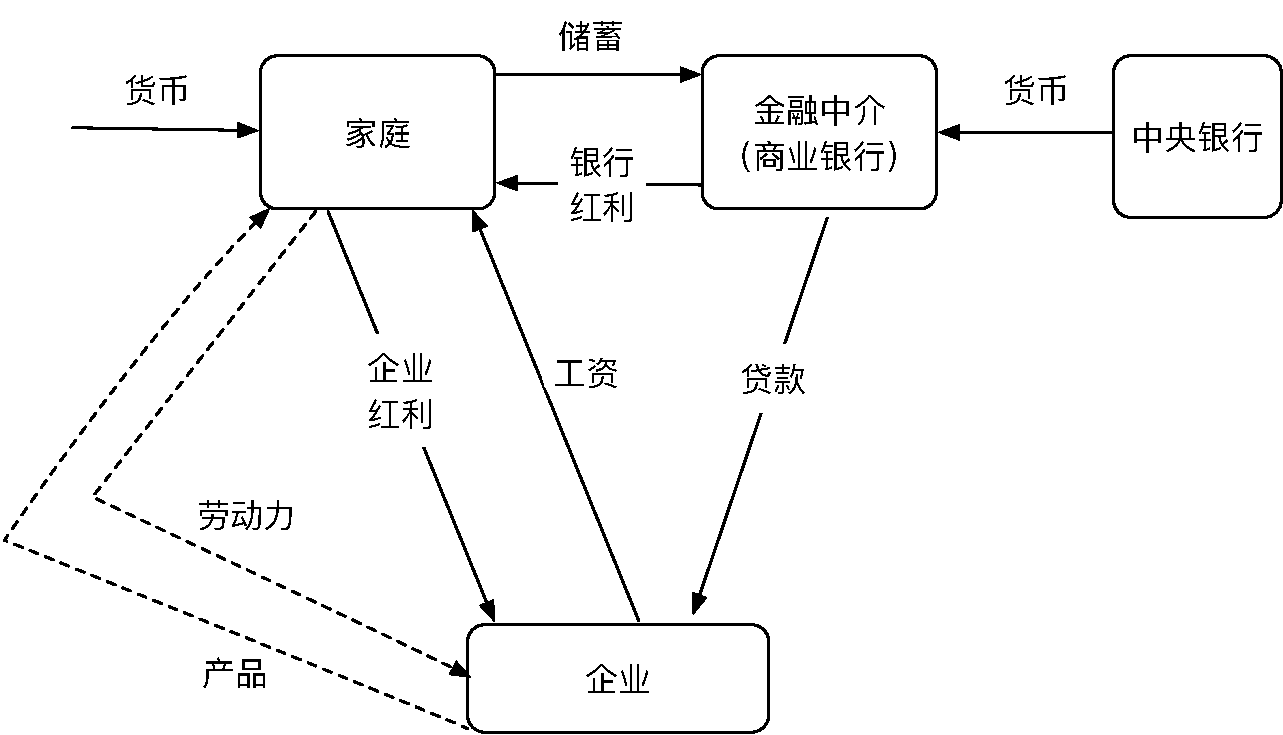
\includegraphics[width=4in]{./figures/20170324-CIA-outline}
 \caption{CIA DSGE模型结构图}
\label{fig:CIA-blueprint}

  \small{注:实线表示名义资金流动。虚线表示实际物质流动。}
\end{figure}

\section{家庭部门}
假定一个永生家庭,追求期望效用的最大化
\begin{equation}
  \label{eq:CIA-hh-max-util}
  \max%_{C_t,H_t,D_t,M_{t+1}}
  E_0 \sum_{t=0}^{\infty} \beta^t \left[ (1-\phi) \cdot \ln C_t + \phi \cdot \ln (1-H_t)\right].
\end{equation}
其中变量$ C_t$表示消费,$0<H_t<1$ 表示劳动时间占全部可支配时间的比重。系数$0<\beta<1$表示时间折旧,$0< \phi <1$表示消费$C_t$相对于休闲$(1-H_t)$,对效用的重要程度。

家庭效用最大化受到2+1个条件限制。

第1个是家庭的现金平衡条件,假定$t$时期家庭需要存留足够数量的现金,以满足同期全部消费需求:
\begin{equation}
  \label{eq:CIA-hh-cash-balance}
  W_t \cdot H_t + M_t - D(t) \ge P_t \cdot C_t,
\end{equation}
其中等式左侧$W_t$表示由市场给定的劳动力平均工资,%$N_t$表示企业部门的劳动力需求,
$M_t$表示$t-1$期末经济体中的基础货币存量,$D_t$表示家庭部门的储蓄,假定储蓄全部以存款形式$D_t$存入银行部门,$M_t$。等式右侧$P_t$表示市场给定的最终产品价格。cash balance是CIA-DSGE模型的核心设定之一。

第2个是家庭的资源约束条件
\begin{equation}
  \label{eq:CIA-hh-rsource-constraint}
  M_{t+1} \ge \left(M_t - D_t + W_t \cdot H_t - P_t \cdot C_t\right) + R_{H,t} \cdot D_t + \left(F_t + B_t\right),
\end{equation}
%等式左侧表示$t$期末经济体中的基础货币存量;
等式右侧分为三个部分。第一部分为现金平衡条件如式\eqref{eq:CIA-hh-cash-balance},第二部分为家庭存款$D_t$的收益,$R_{H,t}$为银行提供给家庭的无风险名义存款利率,第三部分为家庭部门收到的分红\footnote{模型假定银行和企业的资产最终由家庭部门所有,如\cite{Christiano:1992fz}。},分别来自银行部门$B_t$和企业部门$F_t$。根据资源约束条件,$t$期家庭需要决定全部收入中提取多少现金存留在手上,以满足$t$期的消费需求;剩余部分以$D_t$形式存入银行,获取利润,以供$t+1$期消费所用。

第3个是家庭净资产非负条件,假定所有时期家庭的储蓄均大于$0$
\begin{equation}
  \label{eq:CIA-hh-non-negative-deposits-constraint}
  D_t \ge 0.
\end{equation}

\section{企业部门}
假定完全竞争市场环境下,一家典型企业的生产函数
\begin{equation}
  \label{eq:CIA-firm-production-function}
  Y_t = K_t^{\alpha} \cdot (A_t \cdot N_t)^{1-\alpha},
\end{equation}
符合Cobb-Douglas形式。投入要素有2。第1个投入要素为资本存量$K_t$,通过企业往期投资$I_{t-s}, s>0$,经折旧后累积形成,
\begin{equation}
  \label{eq:CIA-firm-capital-accumulation}
  K_{t+1} = I_{t} + (1-\delta) \cdot K_t,
\end{equation}
其中常系数$0<\delta<1$表示自然折旧率。

第2个投入要素为劳动力$N_t$。基于市场给定的名义工资率$W_t$,企业向银行借贷$L_t$,用于支付全部劳动工资
\begin{equation}
  \label{eq:CIA-firm-lending-balance}
  L_t \ge W_t \cdot N_t,
\end{equation}
银行借贷需要支付市场利率$R_{F,t}$。

此外式\eqref{eq:CIA-firm-production-function}中,$\alpha$表示资本的产出弹性。外生变量$A_t$用于描述劳动扩张型技术进步,见第\ref{sec:CIA-exo-shocks}节。

\subsection{生产规模}
如前文所述,完全竞争市场下,利润最大化企业以$R_{F,t}$利率从银行获取贷款$L_t$用于成本支出,即支付员工工资$W_t \cdot N_t$,展开生产。企业将逐渐增加生产规模,直到雇佣额外1单位劳动力的边际收益,等于向银行借贷所需支付的利息。

\begin{equation}
  \label{CIA-firm-optim-partial}
  \frac{\partial \left[ P_t \cdot Y_t - W_t \cdot N_t \right]}{\partial N_t} + \frac{\partial \left[ (1-R_{F,t}) \cdot L_t \right]}{\partial N_t} = 0.
\end{equation}

%设企业追求利润最大化\todo{利润生产和利润使用。利润生产方面,需要补上一段。}。

\subsection{利润的使用}
对于已经生成的利润,$t$期企业核心决策为,决定利润中多少比例留作投资$I_t$,以增加$t+1$期的资本存量$K_{t+1}$,用于扩大再生产;剩余利润以红利$F_t$形式返回家庭部门,用于$t+1$期的消费$C_{t+1}$。企业行为可以表示如下
\begin{equation}
  \label{CIA-firm-max-problem}
  \max E_0 \sum_{t=0}^{\infty} \beta^{t+1} \cdot \frac{F_t}{P_{t+1} \cdot C_{t+1}}.
\end{equation}

企业利润最大化生产活动受到2个条件限制。第1个是预算约束条件,
\begin{equation}
  \label{eq:CIA-firm-budget-constraint}
  P_t \cdot (Y_t-I_t) + L_t \ge F_t + W_t \cdot N_t + R_{F,t} \cdot L_t,
\end{equation}
等式右侧表示全部生产收入和来自银行的贷款;左侧支出部分分别为给家庭部门的红利,劳动力工资,和向银行支付的贷款利息。

第2个是非负借贷条件式\eqref{eq:CIA-firm-lending-balance},确保当期向银行借款数足以支付工资。

\section{银行部门}
类似地,$t$期的银行利润以分红$B_t$形式返还给家庭部门,用于$t+1$期的消费。利润最大化的银行追求
\begin{equation}
  \label{eq:CIA-bank-max-problem}
  \max E_t \sum_{t=0}^{\infty} \beta^{t+1} \cdot \frac{B_{t}}{P_{t+1} \cdot C_{t+1}}.
\end{equation}

银行利润最大化行为受到2个条件限制。第1个是预算约束条件
\begin{equation}
  \label{eq:CIA-bank-budget-constraint}
  B_t + R_{H,t} \cdot D_t \le R_{F,t} \cdot L_t + D_t + X_t - L_t,
\end{equation}
其中$X_t$表示$t$期中央银行对市场释放的基础货币,定义为$t+1$期末基础货币存量和$t$期末基础货币存量的差,
\begin{equation}
  \label{eq:CIA-central-bank-money-injection}
  X_t = M_{t+1} - M_t.
\end{equation}

第2个是资产负债平衡约束,要求同期的银行负债不得超过资产
\begin{equation}
  \label{eq:CIA-bank-balance-sheet}
  X_t + D_t \le L_t.
\end{equation}

\section{一阶条件}
\subsection{家庭部门}
根据最大化式\eqref{eq:CIA-hh-max-util}及约束条件式\eqref{eq:CIA-hh-cash-balance}-\eqref{eq:CIA-hh-non-negative-deposits-constraint},建家庭部门Lagrangian

\begin{align*}
  \mathcal{L} = E_0 \sum_{t=0}^{\infty} \beta^t \cdot & \left\{
\left[(1-\phi) \cdot \ln C_t + \phi \cdot \ln (1-H_t)\right]
   \right. \\
   & \left. + \lambda_t \cdot
   \left[
M_t - D_t + W_t \cdot H_t - P_t \cdot C_t + R_{H,t} \cdot D_t + \left( F_t + B_t - M_{t+1} \right)
   \right]\right\}.
\end{align*}

FOCs:
\begin{align}
  \label{eq:CIA-hh-FOC-C}
  \frac{\partial \mathcal{L}}{\partial C_t} = 0 &\Rightarrow \lambda_t = \frac{1-\phi}{P_t \cdot C_t}, \\
  \label{eq:CIA-hh-FOC-H}
  \frac{\partial \mathcal{L}}{H_t}=0 &\Rightarrow \lambda_t \cdot W_t = \frac{\phi}{1-H_t},\\
  \label{eq:CIA-hh-FOC-M}
  \frac{\partial \mathcal{L}}{\partial M_{t+1}} = 0 &\Rightarrow \frac{\partial \beta \cdot E_t \cdot \left( \lambda_{t+1} \cdot R_{H,t+1} \cdot D_{t+1} \right)}{\partial M_{t+1}} = \lambda_t.
\end{align}

\subsection{企业部门}
利用
将式\eqref{eq:CIA-firm-capital-accumulation}、\eqref{eq:CIA-firm-production-function}
代入\eqref{eq:CIA-firm-budget-constraint}替换$I_t$、$Y_t$,与式  \eqref{eq:CIA-firm-lending-balance}共同构成约束条件
\begin{equation*}
  P_t \cdot \left[
K_t^{\alpha} \cdot \left(A_t \cdot N_t \right)^{1-\alpha} - K_{t+1} + (1-\delta) \cdot K_t
  \right] \ge F_t + W_t \cdot N_t + R_{F,t} \cdot L_t - L_t.
\end{equation*}

建企业部门Lagrangian
\begin{align*}
  \mathcal{L} = E_t \sum_{t=0}^{\infty} \beta^{t+1} \cdot &\left\{ \frac{F_t}{P_{t+1} \cdot C_{t+1}} \right. \\
  &+\left. \lambda_t \cdot \left\{
P_t \cdot \left[ K_t^{\alpha} \cdot \left( A_t \cdot N_t \right)^{1-\alpha} - K_{t+1} + (1-\delta) \cdot K_t \right] - F_t - W_t \cdot N_t - R_{F,t} \cdot L_t + L_t
  \right\} \right\}.
\end{align*}

FOCs:
\begin{align}
  \label{eq:CIA-firm-FOC-F}
  \frac{\partial \mathcal{L}}{\partial F_t} = 0 & \Rightarrow \lambda_t = E_t \frac{1}{P_{t+1} \cdot C_{t+1}}, \\
  \label{eq:CIA-firm-FOC-N}
  \frac{\partial \mathcal{L}}{\partial N_t} = 0 & \Rightarrow P_t \cdot K_{t}^{\alpha} \cdot (1-\alpha) \cdot A_t^{1-\alpha} \cdot N_t^{-\alpha} = W_t,\\
  \label{eq:CIA-firm-FOC-K}
  \frac{\partial \mathcal{L}}{\partial K_{t+1}} = 0 &\Rightarrow \lambda_t \cdot P_t = \beta \cdot E_t \lambda_{t+1} \cdot P_{t+1} \cdot \left[
\alpha \cdot K_{t+1}^{\alpha - 1} \cdot \left( A_{t+1} \cdot N_{t+1} \right)^{1-\alpha} + (1-\delta)
  \right].
\end{align}

\subsection{银行部门}
建立银行部门Lagrangian

\begin{align*}
  \mathcal{L} = E_t \sum_{t=0}^{\infty} \beta^{t+1} \cdot & \left\{ \frac{B_t}{P_{t+1} \cdot C_{t+1}} \right. \\
  &\left.
  + \lambda_t \cdot \left(D_t + R_{F,t} \cdot L_t - R_{H,t} \cdot D_t - L_t + X_t - B_t \right)
  \right\}.
\end{align*}

\subsection{一阶条件的整理}
式\eqref{eq:CIA-hh-FOC-C}代入式\eqref{eq:CIA-hh-FOC-H}以替换$\lambda_t$,可得劳动力供应的决定式
\begin{equation}
  \label{eq:CIA-FOC-labor-supply}
  W_t = \frac{\phi}{1-\phi} \cdot \frac{P_t \cdot C_t}{1-H_t}.
\end{equation}

式\eqref{eq:CIA-hh-FOC-C}代入式\eqref{eq:CIA-hh-FOC-M}以替换$\lambda_t$;结合式\eqref{eq:CIA-bank-budget-constraint}、\eqref{eq:CIA-central-bank-money-injection}可得跨期消费的Euler equation
\begin{equation}
  \label{eq:CIA-FOC-intertemp-consumption-euler}
  \frac{1}{P_t \cdot C_t} = R_{H,t} \cdot \beta \cdot E_t \frac{1}{P_{t+1} \cdot C_{t+1}}.
\end{equation}

\eqref{eq:CIA-firm-FOC-F}代入式\eqref{eq:CIA-firm-FOC-N}以替换$\lambda_t$,可得劳动力需求的决定式
\begin{equation}
  \label{eq:CIA-FOC-labor-demand}
  W_t = \left( 1-\alpha \right) \cdot P_t \cdot K_t^{\alpha} \cdot A_{t}^{1- \alpha} \cdot N_t^{-\alpha}.
\end{equation}

 \eqref{eq:CIA-firm-FOC-F}代入式\eqref{eq:CIA-firm-FOC-K}以替换$\lambda_t$,可得产品市场上跨期消费决策的Euler equation
\begin{equation}
  \label{eq:CIA-FOC-goods}
  E_t \frac{P_t}{P_{t+1} \cdot C_{t+1}} = \beta \cdot E_t \cdot
  \left\{
\left( \frac{P_{t+1}}{P_{t+2} \cdot C_{t+2}} \right) \cdot
\left[
  \alpha \cdot K_{t+1}^{\alpha -1 } \cdot
  \left(A_{t+1} \cdot N_{t+1} \right)^{1-\alpha} + (1-\delta)
\right]
  \right\}.
\end{equation}


\section{市场均衡及部门最优行为}

\subsection{4个市场均衡条件}
假定下述4个完全竞争市场均处于均衡条件,完全出清。

\subsubsection{劳动力市场均衡}

家庭部门的劳动力供应等于企业部门的劳动力需求
\begin{equation}
  \label{eq:CIA-market-clearing-labor}
  H_t = N_t.
\end{equation}

\subsubsection{产品市场均衡}

企业部门的产出完全用于企业再投资和家庭部门的消费
\begin{equation}
  \label{eq:CIA-market-clearing-product}
  Y_t = C_t + I_t.
\end{equation}

\subsubsection{货币市场均衡}

家庭部门对现金(消费)的需求,等于市场上的货币供应
\begin{equation}
  \label{eq:CIA-market-clearing-money}
  P_t \cdot C_t = M_{t+1}.
\end{equation}

\subsubsection{信贷市场均衡}

商业银行的负债等于资产,即式\eqref{eq:CIA-bank-balance-sheet}改写为
\begin{equation}
  \label{eq:CIA-market-clearning-credit}
  X_t + D_t = L_t.
\end{equation}



\subsection{部门最优行为}
将几个市场的均衡行为纳入部门最优行为的决策分析。

\subsubsection{劳动力市场}
劳动力市场均衡条件下,式\eqref{eq:CIA-firm-lending-balance}取等号,可求得平均工资的决定
\begin{equation}
  \label{eq:CIA-wage-determ}
  W_t = \frac{L_t}{N_t}.
\end{equation}

将劳动力市场出清式\eqref{eq:CIA-market-clearing-labor}和均衡工资决定式\eqref{eq:CIA-wage-determ}代入一阶条件式\eqref{eq:CIA-FOC-labor-supply},分别替代$W_t, H_t$可得家庭部门的同期最优消费——劳动供应决策。
\begin{equation}
  \label{CIA-optimal-labor-mkt-intratemp}
  \frac{L_t}{N_t}=\frac{\phi}{1-\phi} \cdot \frac{P_t \cdot C_t}{1-N_t}.
\end{equation}

\subsubsection{产品市场}
产品市场最优条件,见跨期消费平滑Euler equation式\eqref{eq:CIA-FOC-goods}。

\subsubsection{货币市场}
式\eqref{eq:CIA-central-bank-money-injection}代入货币市场均衡条件式\eqref{eq:CIA-market-clearing-money}可得
\begin{equation}
  \label{eq:CIA-market-clearing-money-flow}
  P_t \cdot C_t = M_t + X_t,
\end{equation}
即全部现金需求等于市场上的货币存量和当期新增货币投放量之和。

\subsubsection{信贷市场}
首先由信贷市场均衡式\eqref{eq:CIA-market-clearning-credit}可见,根据银行利润为零的假定
\begin{equation*}
  R_{H,t} \cdot D_t = R_{F,t} \cdot \left(L_t - X_t \right),
\end{equation*}
由此我们有
\begin{equation}
  \label{eq:CIA-interest-rate-unification}
  R_{F,t} = R_{H,t} \equiv R_t.
\end{equation}

式\eqref{eq:CIA-firm-production-function}、\eqref{eq:CIA-wage-determ}和
\eqref{eq:CIA-interest-rate-unification} 代入式\eqref{CIA-firm-optim-partial}分别替换$Y_t, L_t, R_{F,t}$,整理后,可得信贷市场最优条件
\begin{equation}
  \label{CIA-optimal-credit-mkt}
  R_t = \frac{P_t \cdot K_t^{\alpha} \cdot (1-\alpha) \cdot A_t^{1- \alpha} \cdot N_t^{-\alpha}}{W_t}.
\end{equation}

\section{外生冲击}
\label{sec:CIA-exo-shocks}
经济模型中存在两种随机外生冲击。第1种是作用于实体经济部门的劳动增强型技术冲击,假定符合下述形式
\begin{equation}
  \label{eq:CIA-tech-shock}
  \ln A_t = \gamma + \ln A_{t-1} + \varepsilon_{A,t}, \quad \varepsilon_{A,t} \sim \mathcal{N}(0,\sigma_A^2), \quad corr(\varepsilon_{A,t}, \varepsilon_{A,s})=0, \forall s \neq t,
\end{equation}
$\gamma > 0$表示确定性趋势。不可提前预支的当期技术波动用innovation项$\varepsilon_{A,t}$来反映。

由定义式\eqref{eq:CIA-tech-shock}可得外生技术冲击的增速
\begin{equation}
  \label{eq:CIA-tech-shock-growth}
  \frac{A_t}{A_{t-1}} = \exp (\gamma + \varepsilon_{A,t}).
\end{equation}

第2种是作用于非实体非实体经济部门的货币投放增速的冲击。假定货币投放增速表述为
\begin{equation}
  \label{eq:CIA-money-injection-growth-def}
  m_t \equiv \frac{M_{t+1}}{M_t},
\end{equation}
随机冲击符合下述形式
\begin{equation}
  \label{eq:CIA-money-shock}
  \ln m_t = (1-\rho) \cdot \ln m^{*} + \rho \cdot \ln m_{t-1} + \varepsilon_{m,t}, \quad \varepsilon_{m,t} \sim \mathcal{N}(0,\sigma_m^2),  \quad corr(\varepsilon_{m,t}, \varepsilon_{m,s})=0, \forall s \neq t.
\end{equation}
$m^{*}$表示$m_t$的无条件均值。$m^{*}$和$0<\rho<1$一道用于描述常规货币政策,进而二者的变化反映了货币政策的调整。模型引入随机innovation $\varepsilon_{m,t}$表示当期影响货币供应增速变化的波动因素\citep{Sims:1982ks}。

\section{均衡方程组}
\label{sec:CIA-equilibrium-conditions}
模型均衡方程组由9个内生变量和2个外生变量$\{K_{t+1}, N_t, D_t, C_t, L_t, P_t, W_t, Y_t, R_t, A_t/A_{t-1}, m_t\}$共同构成\footnote{有的时候还需要考虑一个派生变量,通货膨胀$\pi_t = \frac{P_t}{P_{t-1}}$。}。对应一组结构方程如下,每个方程的经济学含义在第\ref{sec:CIA-scaling-equilibrium-conditions}节做简要描述:

式\eqref{eq:CIA-wage-determ}、\eqref{CIA-optimal-credit-mkt}代入\eqref{CIA-optimal-credit-mkt}以替代$W_t,R_t$得
  \begin{equation}
    \label{eq:CIA-equil-cond-unscal-inter-euler}
    \frac{1}{P_t \cdot C_t} = \frac{\beta \cdot P_t \cdot K_t^{\alpha} \cdot (1-\alpha) \cdot A_{t}^{1-\alpha} \cdot N_t^{1-\alpha}}{L_t \cdot E_t P_{t+1} \cdot C_{t+1}}.
  \end{equation}

式\eqref{eq:CIA-FOC-goods} $\Rightarrow$
  \begin{equation*}
    E_t \frac{P_t}{P_{t+1} \cdot C_{t+1}} = \beta \cdot E_t \cdot
    \left\{
  \left( \frac{P_{t+1}}{P_{t+2} \cdot C_{t+2}} \right) \cdot
  \left[
    \alpha \cdot K_{t+1}^{\alpha -1} \cdot
    \left(A_{t+1} \cdot N_{t+1} \right)^{1-\alpha} + (1-\delta)
  \right]
    \right\}.
  \end{equation*}

式\eqref{CIA-optimal-labor-mkt-intratemp} $\Rightarrow$
  \begin{equation*}
    \frac{L_t}{N_t}=\frac{\phi}{1-\phi} \cdot \frac{P_t \cdot C_t}{1-N_t}.
  \end{equation*}

式\eqref{eq:CIA-firm-capital-accumulation}、\eqref{eq:CIA-firm-production-function}代入式\eqref{eq:CIA-market-clearing-product}以替换$I_t, Y_t$ $\Rightarrow$
    \begin{equation}
    \label{eq:CIA-equil-cond-unscal-resource}
      K_t^{\alpha} \cdot \left( A_t \cdot N_t \right)^{1-\alpha} = C_t + K_{t+1} - \left( 1 - \delta \right) \cdot K_t.
    \end{equation}

式\eqref{eq:CIA-market-clearing-money} $\Rightarrow$
  \begin{equation*}
    P_t \cdot C_t = M_{t+1}.
  \end{equation*}

式\eqref{eq:CIA-central-bank-money-injection}代入\eqref{eq:CIA-market-clearning-credit}以替代$X_t$ $\Rightarrow$
  \begin{equation}
    \label{eq:CIA-equil-cond-unscal-credit}
    L_t = D_t + M_{t+1} - M_{t}.
  \end{equation}

式\eqref{eq:CIA-firm-production-function} $\Rightarrow$
  \begin{equation*}
    Y_t = K_t^{\alpha} \cdot (A_t \cdot N_t)^{1-\alpha},
  \end{equation*}

式\eqref{eq:CIA-wage-determ} $\Rightarrow$
  \begin{equation*}
    W_t = \frac{L_t}{N_t}.
  \end{equation*}

式\eqref{CIA-optimal-credit-mkt} $\Rightarrow$
  \begin{equation*}
    R_t = \frac{P_t \cdot K_t^{\alpha} \cdot (1-\alpha) \cdot A_t^{1- \alpha} \cdot N_t^{-\alpha}}{W_t}.
  \end{equation*}

外生冲击式\eqref{eq:CIA-tech-shock} $\Rightarrow$
  \begin{equation*}
    \ln A_t = \gamma + \ln A_{t-1} + \varepsilon_{A,t}, \quad \varepsilon_{A,t} \sim \mathcal{N}(0,\sigma_A^2), \quad corr(\varepsilon_{A,t}, \varepsilon_{A,s})=0, \forall s \neq t,
  \end{equation*}

外生冲击式\eqref{eq:CIA-money-shock} $\Rightarrow$
  \begin{equation*}
    \ln m_t = (1-\rho) \cdot \ln m^{*} + \rho \cdot \ln m_{t-1} + \varepsilon_{m,t}, \quad \varepsilon_{m,t} \sim \mathcal{N}(0,\sigma_m^2),  \quad corr(\varepsilon_{m,t}, \varepsilon_{m,s})=0, \forall s \neq t.
  \end{equation*}


\section{去趋势的均衡状态}
\label{sec:CIA-scaling-equilibrium-conditions}
第\ref{sec:CIA-equilibrium-conditions}节的方程组是非平稳的。非平稳来自两方面因素,第一是随机技术冲击和货币冲击的趋势影响。即便假定冲击均为零,第二方面因素在于各变量之间没有统一的稳定状态:实际变量的增速等于$A_t$的增速(除了劳动力$N_t$);名义变量的增速等于$M_t$的增速;总物价水平的增速等于$M_t/A_t$的增速。对上节的变量做去趋势调整:
\begin{equation*}
\begin{cases}
  \text{(名义变量)}&\hat{\mathcal{B}}_t=\frac{\mathcal{B}_t}{A_t} \text{, 其中 } \mathcal{B}_t=[Y_t,C_t,I_t,K_{t+1}]',\\
  \text{(实际变量)}&\hat{\mathcal{C}}_t = \frac{\mathcal{C}_t}{M_t} \text{, 其中 } \mathcal{C}_t=[W_t,D_t,L_t]', \\
  \text{(名义变量)}&\hat{P}_t = \frac{P_t \cdot A_t}{M_t},\\
  \text{(其他)}&\{N_t, R_t\}\text{保持不变,根据式}  \eqref{eq:CIA-money-injection-growth-def}\text{用$m_t - 1$替代$\frac{X_t}{M_t}$}.
\end{cases}
\end{equation*}

由去趋势变量构成的新方程组如下。

式\eqref{eq:CIA-equil-cond-unscal-inter-euler} $\Rightarrow$
\begin{align}
  \frac{1}{\left(\frac{\hat{P}_t \cdot M_{t}}{A_t}\right) \cdot \left(\hat{C}_t \cdot A_t \right)} &=
  \frac{
  \beta \cdot \left(\frac{\hat{P}_t \cdot M_t}{A_t}\right) \cdot \left(\hat{K}_t^{\alpha} \cdot A_{t-1}^{\alpha} \right) \cdot (1-\alpha) \cdot A_t^{1-\alpha} \cdot N_t^{1-\alpha}
  }{
  \left(\hat{L}_t \cdot M_t \right) \cdot E_t \cdot \left(\frac{\hat{P}_{t+1} \cdot M_{t+1}}{A_{t+1}}\right) \cdot \left( \hat{C}_{t+1} \cdot A_{t+1} \right)
  },
  \nonumber \\
  \frac{1}{\hat{P}_t \cdot \hat{C}_t \cdot M_t} &= \frac{
  (1-\alpha) \cdot \beta \cdot \hat{P}_t \cdot M_t \cdot \hat{K}_t^{\alpha} \cdot N_t^{1-\alpha} \cdot \left(\frac{A_t}{A_{t-1}}\right)^{-\alpha}
  }{
  \left(\hat{L}_t \cdot M_t\right) \cdot E_t M_{t+1} \cdot \hat{P}_{t+1} \cdot \hat{C}_{t+1}
  },\nonumber \\
  \label{eq:CIA-equil-cond-scal-inter-euler}
  \frac{1}{\hat{P}_t \cdot \hat{C}_t} &=  \frac{
  (1-\alpha)\cdot \beta \cdot \frac{\hat{P}_t \cdot \hat{K}_t^{\alpha} \cdot N_t^{1-\alpha}}{\hat{L}_t \cdot m_t} \cdot \exp \left[ - \alpha \cdot \left( \gamma + \varepsilon_{A,t} \right)\right]
  }{
  E_t \hat{P}_{t+1} \cdot \hat{C}_{t+1}
  }.
\end{align}
反映信贷市场的最优跨期决策,使得今天放弃1单位消费用于储蓄,导致明天消费增加的现值,等于今天1单位消费带来的满足。

式\eqref{eq:CIA-FOC-goods} $\Rightarrow$
\begin{equation*}
  \frac{P_t}{E_t P_{t+1}\cdot C_{t+1}}
  = \frac{
  \frac{\hat{P}_t \cdot M_t }{A_t}
  }{
  E_t \left(
   \frac{\hat{P}_{t+1} \cdot \hat{M}_{t+1}}{A_{t+1}}
  \right) \cdot \left(
  \hat{C}_{t+1} \cdot A_{t+1}
  \right)
  }
  =\frac{\hat{P}_t}{E_t \hat{P}_{t+1} \cdot \hat{C}_{t+1} \cdot m_t \cdot A_t}
\end{equation*}
进而我们有
\begin{equation*}
  E_t \frac{\hat{P}_t}{\hat{P}_{t+1} \cdot \hat{C}_{t+1} \cdot m_t} = \beta \cdot E_t \frac{\hat{P}_{t+1}}{\hat{P}_{t+2} \cdot \hat{C}_{t+2} \cdot m_{t+1} \cdot \left(\frac{A_{t+1}}{A_t}\right)} \cdot \left[
  \alpha \cdot \hat{K}_{t+1}^{\alpha-1} \cdot N_{t+1}^{1-\alpha} \cdot
  \left(\frac{A_{t+1}}{A_t}\right)^{1-\alpha} + \left( 1-\delta \right)
  \right],
\end{equation*}
\begin{align}
  \label{eq:CIA-FOC-goods-scal}
 E_t \frac{\hat{P}_t}{\hat{P}_{t+1} \cdot \hat{C}_{t+1} \cdot m_t} = \beta \cdot E_t \frac{
 \hat{P}_{t+1}
 }{
 \hat{P}_{t+2} \cdot \hat{C}_{t+2} \cdot m_{t+1}
 } \cdot & \left\{
\alpha \cdot \hat{K}_{t+1}^{\alpha -1} \cdot N_{t+1}^{ 1-\alpha} \cdot \exp \left[-\alpha \cdot \left(\gamma + \varepsilon_{A,t+1}\right)\right] \right.\nonumber \\
& \left. + \left( 1-\delta \right) \cdot \exp \left[ -1 \cdot \left( \gamma + \varepsilon_{A,t+1} \right) \right] \right\}.
\end{align}
反映产品市场的跨期最优决策,确保经济体整体的跨期消费平滑。

式\eqref{CIA-optimal-labor-mkt-intratemp} $\Rightarrow$
\begin{equation}
  \label{CIA-optimal-labor-mkt-intratemp-scal}
  \frac{\hat{L}_t}{N_t}=\frac{\phi}{1-\phi} \cdot \frac{\hat{P}_t \cdot \hat{C}_t}{1-N_t}.
\end{equation}
反映劳动力市场的当期最优决策:家庭部门的劳动力供应(企业部门的劳动力需求),和消费——休闲边际替代率之间的关系。

式\eqref{eq:CIA-equil-cond-unscal-resource} $\Rightarrow$
\begin{equation}
  \label{eq:CIA-equil-cond-scal-resource}
  \hat{K}_t^{\alpha} \cdot N_t^{1-\alpha} \cdot \exp \left[ -\alpha \cdot \left( \gamma + \varepsilon_{A,t} \right) \right] = \hat{C}_t + \hat{K}_{t+1} -  (1-\delta) \cdot \hat{K}_t \cdot \exp \left[
  -1 \cdot \left( \gamma + \varepsilon_{A,t} \right)
  \right].
\end{equation}
反映总量上的资源约束条件:当期产出全部用于当期消费和当期投资;当期投资贡献于下一期的资本存量积累。

式\eqref{eq:CIA-market-clearing-money} $\Rightarrow$
\begin{equation}
  \label{eq:CIA-market-clearing-money-scal}
  \hat{P}_t \cdot \hat{C}_t = m_t.
\end{equation}
反映货币市场的最优决策:货币的名义消费需求等于名义货币供应量。名义货币供应量等于名义现有货币存量与当期货币注入量之和。

式\eqref{eq:CIA-equil-cond-unscal-credit} $\Rightarrow$
\begin{equation}
  \label{eq:CIA-equil-cond-scal-credit}
  \hat{L}_t = \left( m_t - 1 \right) + \hat{D}_t.
\end{equation}
反映信贷市场的最优决策:商业银行追求资产——负债平衡。

式\eqref{eq:CIA-firm-production-function} $\Rightarrow$
\begin{equation}
  \label{eq:CIA-firm-production-function-scal}
  \hat{Y}_t = \hat{K}_t^{\alpha} \cdot N_t^{1-\alpha} \cdot \exp \left[ - \alpha \cdot \left( \gamma + \varepsilon_{A,t} \right) \right].
\end{equation}
反映经济整体的投入产出关系。

式\eqref{eq:CIA-wage-determ} $\Rightarrow$
\begin{equation}
  \label{eq:CIA-wage-determ-scal}
  \hat{W}_t = \frac{\hat{L}_t}{N_t}.
\end{equation}
反映企业对商业银行的贷款需求,与企业生产活动中的劳动力需求(家庭部门的劳动力供应)之间的关系。

式\eqref{CIA-optimal-credit-mkt} $\Rightarrow$
\begin{equation}
  \label{CIA-optimal-credit-mkt-scal}
  R_t = \left( 1-\alpha \right) \cdot \frac{\hat{P}_t \cdot \hat{K}_t^{\alpha} \cdot N_t^{1 - \alpha}}{\hat{L}_t} \cdot \exp \left[ -\alpha \cdot \left( \gamma + \varepsilon_{A,t} \right) \right].
\end{equation}
反映信贷市场的最优决策:均衡利率水平表示额外1单位劳动力投入的边际产出效果,等于借贷用于雇佣此额外1单位劳动力所需支付的成本。

外生技术冲击和货币冲击,如式\eqref{eq:CIA-tech-shock-growth}、\eqref{eq:CIA-money-shock}所示。

此外,实际观测到的经济增速和稳定状态下的经济增速之间的关系如下
\begin{equation}
  \label{eq:CIA-gdp-growth-obs-stab}
  \frac{Y_t}{Y_{t-1}}=\frac{\hat{Y}_t}{\hat{Y}_{t-1}} \cdot \exp \left( \gamma + \varepsilon_{A,t} \right).
\end{equation}

类似地,实际观测到的通货膨胀和稳定状态下的通货膨胀之间关系如下
\begin{equation}
  \label{eq:CIA-inflation-obs-stab}
  \frac{P_t}{P_{t-1}} = \frac{\hat{P}_{t}}{\hat{P}_{t-1}} \cdot m_{t-1} \cdot \exp \left[ -1 \cdot \left( \gamma + \varepsilon_{A,t} \right) \right]
\end{equation}
